% \counterwithout{section}{chapter}

\vspace{3mm}
\noindent \textbf{Lecture 2 --- January 23\rd}

\section{The Structuring of Protest}
At the heart of sociology, there is an ongoing debate between the importance of agency and structure.
Agency is defined to be the capacity of human beings to act independently.
Structuralism is a branch of sociological belief that emphasizes that agency is shaped and constrained by the structures of society.
One can think of this debate as a continuum, where all sociologists lay in some point, giving more or less important to agency and structure.

\begin{center}
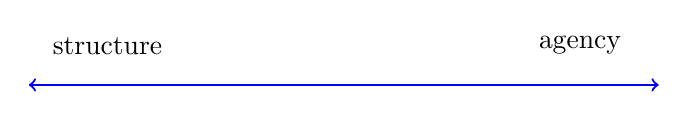
\begin{tikzpicture}
    \draw[thick, <->, blue] (0,0)  -- (8, 0);
    \draw (1, 0.5) node{structure};
    \draw (7, 0.5) node{agency};
    \draw[.] (5,0);
\end{tikzpicture}
\end{center}

Q: Is agency required for structure to arise?

Piven and Cloward make a structuralist argument regarding social movements.
More specifically, they argue that the structure of society influences when movements can arise, what shape the movements will take, and how effective they will be.

\begin{center}
\textit{``In seeking to do what wasn't possible, we failed to do what was... (p. TODO)''}
\end{center}

Notably, Piven \& Cloward offer their own ideas of what a social movement is.
In other words, what should count as a social movement (pp. 3-4).
The two main criteria that they propose are that there should be (a) a transformation of consciousness, and (b) a transformation of behavior.

\subsection{Transformation of Consciousness}
We summarize the criteria that Piven \& Cloward give for a transformation of consciousness below:
\begin{enumerate}
    \item \textit{The system loses legitimacy:}
    In other words, people view the structure of society as unjust and wrong.
    This should not be surprising.
    In fact, most people, at most points in time, believe that society is unjust and wrong (at least to some extent).
    However, this is still an important and necessary condition for a social movement to arise (at least according to Piven \& Cloward).
    \item \textit{Alternatives seem possible:}
    Unlike most of the time, people think that there indeed does exist another way of living.
    \item \textit{Sense of efficacy:}
    Finally, the people come to believe that not only is the system wrong and that there exists a viable alternative, but that this alternative is indeed something that is attainable.
\end{enumerate}
There is a sort of implicit precedence between these three criteria.
Before people think that they can change their living situation to something better, they must have an idea of what the alternative is in mind, and before people conceive that alternative, it is necessary that they see something that is wrong and requires change within their current conditions.

\subsection{Transformation of Behavior}

\begin{enumerate}
    \item \textit{Masses of people become defiant:}
    By this, we mean that people begin to break the rules and norms established in society.
    These can be formal rules (such as the law), or cultural rules.
    Not all movements break the law, but all movements break some form of social norm.
    \item \textit{Defiance is acted out collectively:}
    It is not only necessary that rules and norms are broken by the people, but that people engaging in this disobedience also believe that they are acting as part of a larger group or movement.
\end{enumerate}
Succinctly, we can say 
\begin{center}
\textit{``A protest movement is collective defiance fueled by a transformation of consciousness.''}  
\end{center}


\section{Emergence of Protest Movements}
Now that we have discussed \textit{what} social movements are, a natural question to ask is \textit{when} social movements \textbf{emerge}.
Piven \& Cloward give a characterization for the conditions necessary to spark a social movement.

\begin{enumerate}
    \item \textit{Massive social or economic changes:}
    There must be a rapid and drastic change in the living conditions of a large group of people.
    This can be a massive migration, industrialization, depression, or any other number of such large-scale events.
    \item \textit{Institutional breakdown:}
    The aforementioned massive social/economic changes begin to strain the institutions.
    For example, an economic force like a depression can put a lot of strain on a number of institutions.
    This, importantly, disrupts the routines of people's daily lives.
    \item \textit{Transformation of consciousness:} 
    These two conditions put together, cause a profound \textbf{social dislocation}.
    Informally, people's lives are thrown out of whack.
    This is often sufficient to cause a transformation of consciousness, of the kind we had defined and talked about at length previously.
    \item \textit{Division \& competition among elites:}
    The vested interest of the ruling class is in preserving the status quo.
    Mostly, they are unified in their interest in maintaining the status quo.
    Nonetheless, periods of massive economic change and social upheaval can create fissures among the elite class.
    This can cause dissonance and delegitimize their authority.

\end{enumerate}
Once again, Piven \& Cloward provide us with a fancy quote to characterize these criteria:
\begin{center}
\textit{``The social arrangements that are ordinarily perceived as just and immutable must come to be perceived as unjust and mutable (p. TODO).''}
\end{center}
